\documentclass{article}
\usepackage[utf8x]{inputenc}
\usepackage{ucs}
\usepackage{amsmath} 
\usepackage{amsfonts}
\usepackage{marvosym}
\usepackage{wasysym}
\usepackage{upgreek}
\usepackage[english,russian]{babel}
\usepackage{graphicx}
\usepackage{float}
\usepackage{textcomp}
\usepackage{hyperref}
\usepackage{geometry}
  \geometry{left=2cm}
  \geometry{right=1.5cm}
  \geometry{top=1cm}
  \geometry{bottom=2cm}
\usepackage{tikz}
\usepackage{ccaption}
\usepackage{multicol}
\usepackage{fancyvrb}

\usepackage{listings}
%\setlength{\columnsep}{1.5cm}
%\setlength{\columnseprule}{0.2pt}

\usepackage{colortbl,graphicx,tikz}
\definecolor{X}{rgb}{.5,.5,.5}

\title{ДЗ. Работа с изображениями в формате \texttt{.ppm}}
\date{}
\begin{document}
\pagenumbering{gobble}

\lstset{
  language=C++,                % choose the language of the code
  basicstyle=\linespread{1.1}\ttfamily,
  columns=fixed,
  fontadjust=true,
  basewidth=0.5em,
  keywordstyle=\color{blue}\bfseries,
  commentstyle=\color{gray},
  stringstyle=\ttfamily\color{orange!50!black},
  showstringspaces=false,
  %numbers=false,                   % where to put the line-numbers
  numbersep=5pt,
  numberstyle=\tiny\color{black},
  numberfirstline=true,
  stepnumber=1,                   % the step between two line-numbers.        
  numbersep=10pt,                  % how far the line-numbers are from the code
  backgroundcolor=\color{white},  % choose the background color. You must add \usepackage{color}
  showstringspaces=false,         % underline spaces within strings
  captionpos=b,                   % sets the caption-position to bottom
  breaklines=true,                % sets automatic line breaking
  breakatwhitespace=true,         % sets if automatic breaks should only happen at whitespace
  xleftmargin=.2in,
  extendedchars=\true,
  keepspaces = true,
}
\lstset{literate=%
   *{0}{{{\color{red!20!violet}0}}}1
    {1}{{{\color{red!20!violet}1}}}1
    {2}{{{\color{red!20!violet}2}}}1
    {3}{{{\color{red!20!violet}3}}}1
    {4}{{{\color{red!20!violet}4}}}1
    {5}{{{\color{red!20!violet}5}}}1
    {6}{{{\color{red!20!violet}6}}}1
    {7}{{{\color{red!20!violet}7}}}1
    {8}{{{\color{red!20!violet}8}}}1
    {9}{{{\color{red!20!violet}9}}}1
    {~} {$\sim$}{1}
}


\title{Семинар \#2: Инкапсуляция. Классные задачи.\vspace{-5ex}}\date{}\maketitle
\section*{Инкапсуляция}
Инкапсуляция -- это размещение в классе/структуре данных и функций, которые с ними работают. Структуру с методами можно называть классом. Переменные класса называются полями, а функции класса -- методами.
\begin{multicols}{2}\setlength{\columnseprule}{0.4pt}
\textbf{Без инкапсуляции:}
\begin{lstlisting}
#include <cmath>
#include <iostream>

struct Point {
    float x, y;
};

float norm(const Point& p) {
    return sqrt(p.x*p.x + p.y*p.y);
}

void normalize(Point& p) {
    float pnorm = norm(p);
    p.x /= pnorm;
    p.y /= pnorm;
}

Point operator+(const Point& l, 
                        const Point& r) {
    Point result = {l.x + r.x, l.y + r.y};
    return result;
}

int main() {
    Point p = {1, 2};
    normalize(p);
    std::cout << p.x << " " 
              << p.y << std::endl;
}

\end{lstlisting}

\textbf{С инкапсуляцией:}
\begin{lstlisting}
#include <cmath>
#include <iostream>

struct Point {
    float x, y;

    float norm() const {
        return sqrt(x*x + y*y);
    }

    void normalize() {
        float pnorm = norm();
        x /= pnorm;
        y /= pnorm;
    }

    Point operator+(const Point& r) const {
        Point result = {x + r.x, y + r.y};
        return result;
    }
};

int main() {
	Point p = {1, 2};
	p.normalize();
	std::cout << p.x << " " 
	          << p.y << std::endl;
}
\end{lstlisting}
\end{multicols}
Обратите внимание на следующие моменты:
\begin{itemize}
\item[--] Методы имеют прямой доступ к полям \texttt{x} и \texttt{y}. Передавать саму структуру(или ссылку на неё) в методах не нужно.
\item[--] Вызов метода класса осуществляется с помощью оператора \texttt{.}(точка).
\item[--] Спецификатор \texttt{const} после объявления метода (например, \texttt{float norm() const}) означает, что этот метод не будет менять поля.
Желательно указывать этот спецификатор для всех методов, которые не изменяют объект.
\item[--] При перегрузке бинарных операций объектом является левый аргумент, а параметром функции -- правый. Т.е. \texttt{p + q} превратится в \texttt{p.operator+(q)}.
\end{itemize}

\textbf{Задача 1:} Сделайте задание в файлах \texttt{0point\_without\_encapsulation.cpp}, \texttt{1point\_with\_encapsulation.cpp} и 
\texttt{2point\_separate\_definition.cpp}

\newpage

\subsection*{Модификаторы доступа \texttt{public} и \texttt{private}}
Модификаторы доступа служат для ограничения доступа к полям и методам класса.
\begin{itemize}
\item[--] \texttt{public} -- поля и методы могут использоваться где угодно
\item[--] \texttt{private} -- поля и методы могут использовать только методы этого класса и друзья (особые функции и классы, объявленные с использованием ключевого слова \texttt{friend})
\end{itemize}
\textbf{Задача 2:} Сделайте задание в файле \texttt{3point\_public\_private.cpp}
\subsection*{Конструкторы}
Конструктор -- это специальный метод, который вызывается автоматически при создании экземпляра класса.
\begin{lstlisting}
struct Point {
private:
	float x, y;
public:
	// Конструктор:
	Point(float ax, float ay) {
		x = ax;
		y = ay;
	}
	// другие методы
};
int main() {
	// Если несколько разных синтаксов создания экземпляра класса с вызовом конструктора:
	Point a = Point(7, 3);
	Point b(7, 3);
	Point c = {7, 3};
	Point d {7, 3};
	// Все они делают одно и то же - создают переменную на стеке и вызывают конструктор
	// В современном C++ предпочтительным является способ d
}
\end{lstlisting}
Особым видом конструктора является конструктор копирования:
\begin{lstlisting}
Point(const Point& p)
\end{lstlisting}
Он используется для создание нового экземпляра класса по уже имеющемуся экземпляру.\\
\textbf{Задача 3:} Сделайте задание в файле \texttt{4point\_constructors.cpp}

\subsection*{Ключевое слово \texttt{this} и оператор присваивания}
Ключевое слово \texttt{this} - это указатель на экземпляр класса, который можно использовать в методах этого класса.\\
Оператор присваивания -- это просто перегруженный оператор \texttt{=}. Оператор присваивания должени вернуть ссылку на текущий объект, то есть \texttt{*this}.\\

Нужно различать оператор присваивания и вызов конструктора:
\begin{lstlisting}
Point a = Point(7, 3);  // Конструктор ( оператор присваивания не вызывается )
Point b = a;            // Конструктор копирования ( оператор присваивания не вызывается )
Point c;                // Конструктор по умолчанию
c = a;                  // Оператор присваивания
\end{lstlisting}
Оператор присваивания должен возвращать ссылку на левый аргумент\\
\textbf{Задача 4:} Сделайте задание в файлах \texttt{6point\_this.cpp}, \texttt{7point\_copy\_constructor.cpp} и \texttt{9point\_default.cpp}.

\newpage
\section*{Создаём свой класс строки}
Строки в языке \texttt{C} представляют собой просто массивы с элементами типа \texttt{char}(однобайтовое число). Работать с такими строками не очень удобно. Нужно выделять и удалять необходимую память, следить за тем, чтобы строка помещалась в эту память на всём этапе выполнения программы, для работы со этими строками нужно использовать специальные функции из библиотеки \texttt{string.h}. Это всё может привести к ошибкам. В этом разделе мы создадим класс \texttt{String} -- класс строки, с которым удобнее и безопаснее работать, чем со строками в стиле \texttt{C}. Заготовка класса выглядит так:
\begin{lstlisting}
#include <cstdlib>
class String {
private:
	unsigned int size;
	char* data;
public:
	String(const char* str) {
		// Находим размер строки str (strlen не будем пользоваться)
		size = 0;
		while (str[size])
			size++;
		// Выделяем память
		data = (char*)malloc(sizeof(char) * (size + 1));
		// Копируем массив str в новый массив data
		for (int i = 0; str[i]; i++)
			data[i] = str[i];
		data[size] = '\0';
	}
	unsigned int get_size() const {
		return size;
	}
	const char* c_str() const {
		return data;
	}
};
int main() {
	String a = "Elephant"; // Создаём экземпляр класса String, используя конструктор
}
\end{lstlisting}

Схематично это можно представить следующим образом:
\begin{center}
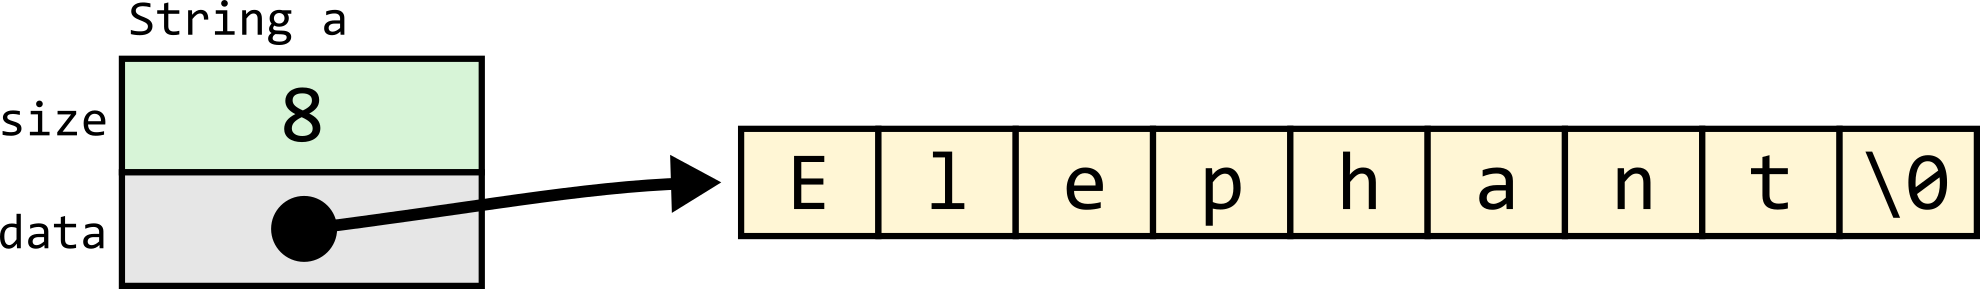
\includegraphics[scale=0.86]{../images/string_base.png}
\end{center}

\textbf{Задача 5:} Сделайте задание в файлах \texttt{00string.cpp} и \texttt{01string\_constructor.cpp}.
\newpage
\subsection*{Деструктор}
В коде выше выделяется память для массива \texttt{data}. Эта память выделяется при вызове конструктора (то есть при создании объекта). Однако она нигде не освобождается. Освободить её вручную мы не можем, так как поле \texttt{data} является приватным и это бы противоречило принципу сокрытия данных. Эта память должна освобождаться автоматически при удалении объекта.
\begin{lstlisting}
~ String() {
	free(data);
}
\end{lstlisting}
\textbf{Задача 6:} Сделайте задание в файлах \texttt{02string\_destructor.cpp} и \texttt{03string\_destructor\_order.cpp}.

\subsection*{Операторы \texttt{new} и \texttt{delete}}
Использовать \texttt{malloc} и \texttt{free} для создания объектов с конструкорами и деструкторами в куче не получится.\\
\texttt{malloc} просто выделяет память и не вызывает никаких конструкторов\\
\texttt{free} просто освобождает память и не вызывает никаких деструкторов\\
Для выделения памяти в куче с вызовом конструктора используется оператор \texttt{new}:
\begin{lstlisting}
String* p = new String("Hippo");
\end{lstlisting}
Для освобождения памяти в куче с вызовом деструктора используется оператор \texttt{delete}.

\begin{center}
\begin{tabular}{c}
\begin{lstlisting}
new = malloc + конструктор
delete = free + деструктор
\end{lstlisting}
\end{tabular}
\end{center}

\textbf{Задача 7:} Сделайте задание в файлах \texttt{04string\_new\_delete.cpp} и \texttt{05new\_delete.cpp}.

\subsection*{Перегруженные операторы класса \texttt{String}}
\begin{itemize}
\item \textbf{Оператор сложения:} \texttt{String operator+(const String\& right) const} \\
Этот оператор должен создавать новый экземпляр, задавать его поля (в частности придётся выделить память под строку-сумму) и возвращать этот экземпляр.

\item \textbf{Оператор присваивания сложения:} \texttt{String\& operator+=(const String\& right)}\\
Этот оператор не должен создавать новый экземпляр. Он должен изменять левый операнд (т. е. сам объект), и возвращать ссылку на этот объект (т. е. \texttt{*this}).

\item \textbf{Оператор присваивания:} \texttt{String\& operator=(const String\& right)}\\
Этот оператор не должен создавать новый экземпляр. Он должен изменять левый операнд (т. е. сам объект), так чтобы он стал идентичен правому. Если размеры строк не совпадают, то в данной реализации строки вам придётся удалить память левой строки и снова выделить память нужного размера. При этом нужно отдельно рассмотреть случай когда левый и правый операнд это один и тот же объект. 
\begin{lstlisting}
String a {"Cat"};
a = a;
\end{lstlisting}
Конечно, в этом случае ничего удалять не нужно.

\item \textbf{Оператор сравнения:} \texttt{bool operator==(const String\& right) const}\\
Этот оператор должен сравнивать строки (массивы \texttt{data}) и возвращать \texttt{true} или \texttt{false}.

\item \textbf{Оператор индексации:} \texttt{char\& operator[](unsigned int i)}\\
Этот оператор должен возвращать ссылку на \texttt{i}-ый символ строки.

\item \textbf{Индексация с проверкой на выход за границы:} \texttt{char\& at(unsigned int i)}\\
Этот метод должен проверять, что индекс \texttt{i} не выходит за границы диапазона и, если это так, возвращать ссылку на \texttt{i}-ый символ строки. Иначе, этот метод должен печатать сообщение об ошибке и завершать программу.
\end{itemize}
\textbf{Задача 8:} Сделайте задание в файлах \texttt{06string\_operators.cpp} и \texttt{07string\_operator[].cpp}.

\newpage
\section*{Раздельная компиляция класса}
Методы можно вынести из определения класса следующим образом:
\begin{multicols}{2}\setlength{\columnseprule}{0.4pt}
\textbf{Определение методов в теле класса:}
\begin{lstlisting}
#include <cmath>
#include <iostream>


struct Point {
    float x, y;

    float norm() const {
        return sqrt(x*x + y*y);
    }

    void normalize() {
        float pnorm = norm();
        x /= pnorm;
        y /= pnorm;
    }

    Point operator+(const Point& r) const {
        Point result = {x + r.x, y + r.y};
        return result;
    }
};





int main() {
	Point p = {1, 2};
	p.normalize();
	std::cout << p.x << " " 
              << p.y << std::endl;
}
\end{lstlisting}
\vfill\null
\columnbreak

\textbf{Определение методов вне тела класса:}
\begin{lstlisting}
#include <cmath>
#include <iostream>

struct Point {
    float x, y;

    float norm() const;
    void normalize();
    Point operator+(const Point& r) const;
};

float Point::norm() const {
    return sqrt(x*x + y*y);
}

void Point::normalize() {
    float pnorm = norm();
    x /= pnorm;
    y /= pnorm;
}

Point Point::operator+(const Point& r) const{
    Point result = {x + r.x, y + r.y};
    return result;
}

int main() {
	Point p = {1, 2};
	p.normalize();
	std::cout << p.x << " " 
              << p.y << std::endl;
}
\end{lstlisting}
\end{multicols}

Теперь эти методы можно скомпилировать отдельно. Для этого их нужно вынести в отдельный компилируемый файл \texttt{point.cpp}, а определение класса в отдельный файл \texttt{point.h}. Так называемый заголовочный файл \texttt{point.h} нужен, так как определение класса нужно и файле \texttt{point.cpp} и в файле \texttt{main.cpp}. Для компиляции используем:
\begin{verbatim}
g++ main.cpp point.cpp
\end{verbatim}

\begin{center}
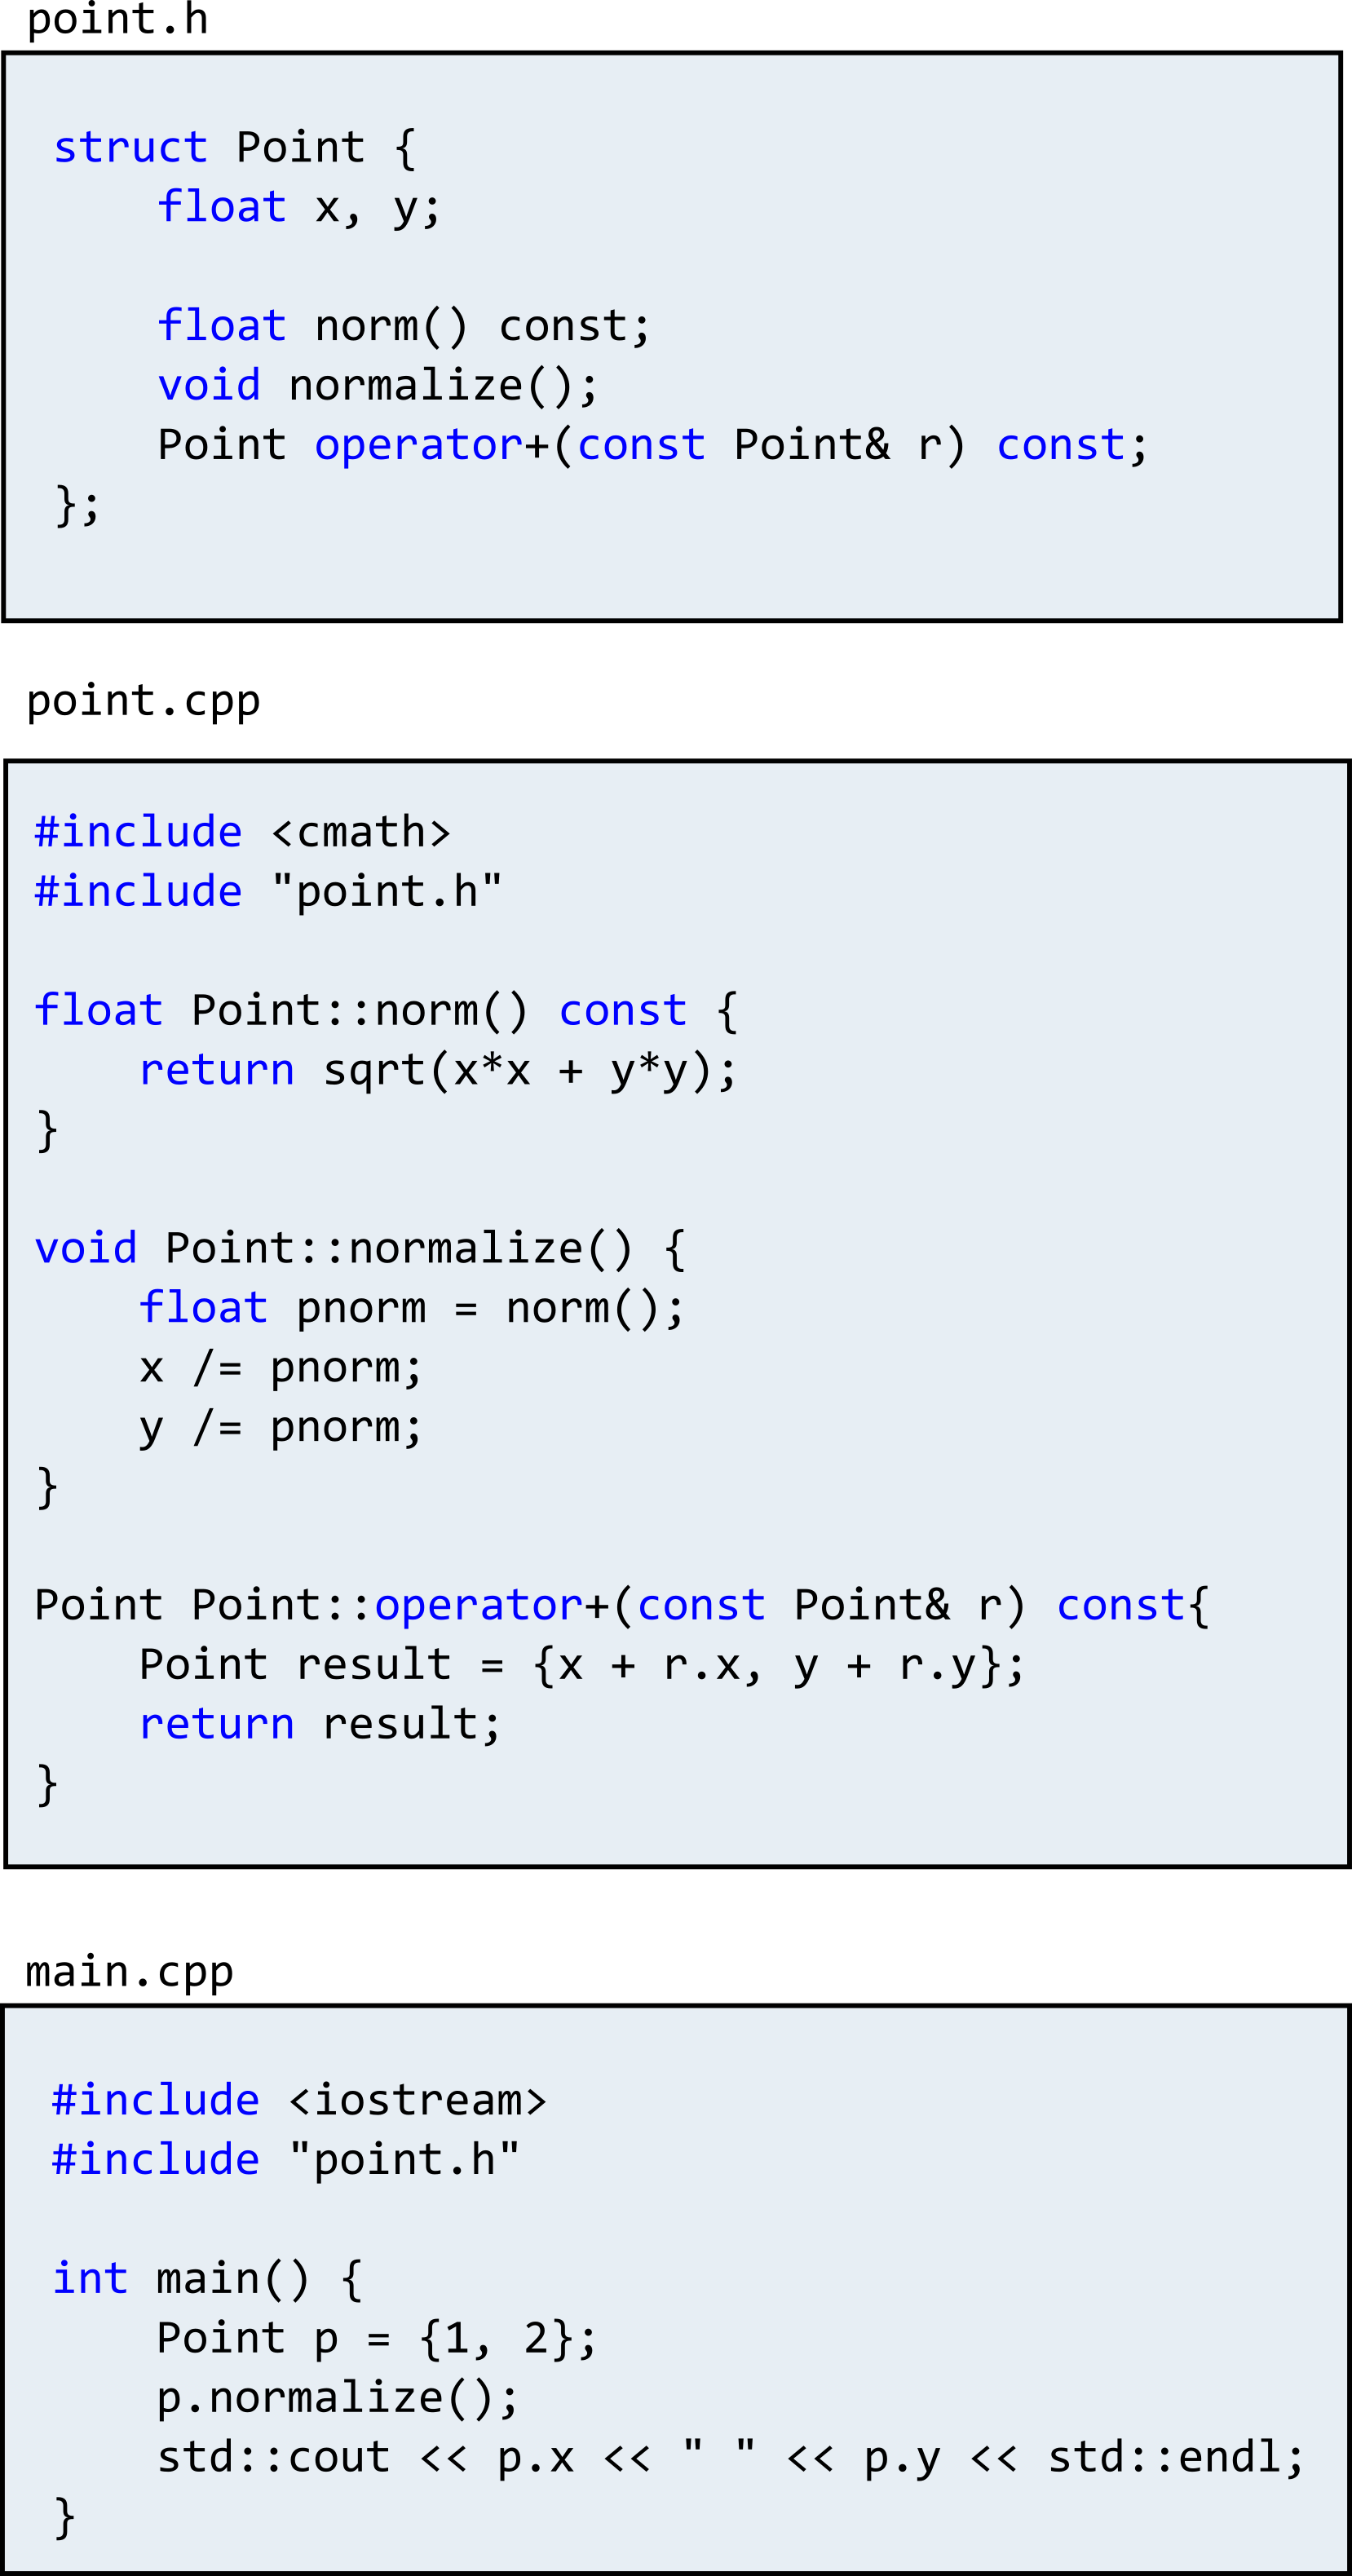
\includegraphics[scale=0.65]{../images/sepcompilation.png}
\end{center}

\subsection*{Задачи:}
\begin{enumerate}
\item Раздельно скомпилируйте класс строки. Для этого создайте файлы \texttt{String.h} и \texttt{String.cpp} и поместите в них объявление класса \texttt{String} и определение его методов соответственно.
\item В папке \texttt{2image} лежит программа, которая работает с классом \texttt{Image} -- классом для работы с изображениями в формате \texttt{ppm}. Сделайте задание в \texttt{main.cpp}.
\end{enumerate}
\end{document}